\noindent Section, figure and table numbers without the prefix S refer to the main paper. Contents: S1 proofs of
Propositions 1--3, Theorems 1--2 and Corollary 1; S2 simulation (Fig.~S1) and why marginal thresholds do not control the
minority class; S3 calibration size, region and gene transfer (Fig.~S2A--C), per-gene coverage (Table~S1) and prior
estimation (Table~S2); S4 strata, assay-label sensitivity (Table~S3) and calls judged against ClinVar labels
(Table~S4); S5 implementation.

\section{Proofs}\label{app:proofs}
Assumptions, propositions, theorems and the corollary are stated in \cref{sec:theory}; $Q$, $C$, $\hat t_k$, $L^+$
and $U^-$ are defined in \cref{sec:method}.


Throughout, fix a class $k$ and write $F_k$ for the distribution function of the nonconformity $r_k$ of a variant drawn
from $Q(\cdot\mid Y=k)$. By Assumption 1, the kept calibration variants (one per residue of $\mathcal A$)
and the variant to be called are independent draws from $Q$; conditionally on all labels, the $n_k$ kept variants of
class $k$ and a class-$k$ test variant are independent draws from $Q(\cdot\mid Y=k)$.

\paragraph{Proposition 1.}
Conditionally on the labels, the $n_k+1$ nonconformities of the class-$k$ kept variants and of the test variant are
exchangeable, so with ties broken at random the rank of the test value is uniform on $\{1,\dots,n_k+1\}$
\cite{Vovk2005,Angelopoulos2023}. The test value is at most the $j_k$-th smallest calibration value with probability
$j_k/(n_k+1)$, which lies in $[1-\alpha_k,\,1-\alpha_k+1/(n_k+1))$ for $j_k=\lceil (n_k+1)(1-\alpha_k)\rceil$; ties only
increase the probability, which gives the lower bound in general. If $j_k>n_k$ then $\hat t_k=\infty$. Since $k\in C$
exactly when $r_k\le\hat t_k$, the claim follows. \hfill$\square$

\paragraph{Proposition 2.}
Conditionally on the labels, the coverage of the threshold is $F_k(\hat t_k)=F_k(r^{(k)}_{(j)})$. If $F_k$ is continuous,
$F_k(r^{(k)}_{(j)})$ is the $j$-th order statistic of $n_k$ independent uniforms and has the
$\mathrm{Beta}(j,n_k-j+1)$ distribution, so $\Pr\{F_k(\hat t_k)<1-\alpha_k\}=F_{\mathrm{Beta}(j,n_k-j+1)}(1-\alpha_k)\le\delta$
by the choice of $j_k$ \cite{Vovk2013}. If $F_k$ has atoms, write $r=F_k^{-1}(U)$ with $U$ uniform and
$F_k^{-1}$ the generalized inverse; then $r^{(k)}_{(j)}=F_k^{-1}(U_{(j)})$ and $F_k(F_k^{-1}(u))\ge u$, so
$F_k(r^{(k)}_{(j)})\ge U_{(j)}$ and the bound still holds. If no $j\le n_k$ qualifies, $\hat t_k=\infty$ and coverage
is 1. \hfill$\square$

\paragraph{Proposition 3.}
Fix $\mathcal A$. Both ranks in \eqref{eq:rank} are non-increasing in $\alpha$ (the in-expectation rank because
$\lceil (n_k+1)(1-\alpha)\rceil$ is, the PAC rank because $F_{\mathrm{Beta}(j,n_k-j+1)}(1-\alpha)$ increases in $\alpha$
for each $j$), so $\hat t_k(\alpha)$ is non-increasing in $\alpha$ and the set $\{r_k\le\hat t_k(\alpha)\}$ shrinks as
$\alpha$ grows. Hence, for any $\hat\alpha\in G$ that depends on $\mathcal B$ but not on the test variant,
$\Pr(k\in C_{\hat\alpha}\mid Y=k,\mathcal A,\mathcal B)\ge\Pr(k\in C_{\max G}\mid Y=k,\mathcal A)$, and taking
expectations over $\mathcal A$ and Proposition~1 at $\alpha_k=\max G$ give the first claim. For the PAC rank at level
$\delta/|G|$, Proposition~2 applied to each $\alpha\in G$ and a union bound give, with probability at least $1-\delta$,
coverage at least $1-\alpha$ for every $\alpha\in G$ simultaneously, in particular for $\hat\alpha$. \hfill$\square$

\paragraph{Theorem 1.}
The thresholds $\hat t(\alpha)$ depend only on $\mathcal A$ and are fixed given $\mathcal A$. Conditionally on
$\mathcal A$ and on the labels of the kept variants of $\mathcal B$, the class-1 kept variants of $\mathcal B$ are
$n_1$ independent draws from $Q(\cdot\mid Y=1)$, so the number of them called LoF is
$\mathrm{Binomial}(n_1,\mathrm{TP}(\alpha))$ with $\mathrm{TP}(\alpha)=\Pr(\text{call LoF}\mid Y=1)$, and likewise for the
other three counts. Each one-sided Clopper--Pearson bound \cite{ClopperPearson1934} at level $\delta/(2|G|)$ fails with
probability at most $\delta/(2|G|)$; the conventions for $x=0$, $x=n$ and $n=0$ in Section 3 give the trivial
bounds 0 and 1, which never fail. For $\mathrm{LR}^+$ there are $2|G|$ such bounds ($\ell_{\mathrm{TP}}$ and
$u_{\mathrm{FP}}$ for each $\alpha$), so by the union bound all of them hold simultaneously with probability at
least $1-\delta$. On that event $\mathrm{TP}(\alpha)\ge\ell_{\mathrm{TP}}(\alpha)$ and
$\mathrm{FP}(\alpha)\le u_{\mathrm{FP}}(\alpha)$ for every $\alpha\in G$, hence
$\mathrm{LR}^+(\hat t(\alpha))\ge L^+(\alpha)$ for every $\alpha$ (with $\mathrm{LR}^+=\infty$ when
$\mathrm{FP}(\alpha)=0$), including any $\hat\alpha^+$ chosen from these data. Since this probability bound holds for
every $\mathcal A$, it also holds unconditionally. The argument for $\mathrm{LR}^-$ is identical with $u_{\mathrm{FN}}$ and $\ell_{\mathrm{TN}}$.
The event does not involve the levels $\tau$, so it covers every evidence level reported. \hfill$\square$

\paragraph{Theorem 2.}
Fix $\mathcal A$, so the thresholds and the hypotheses $H_\alpha:\mathrm{LR}^+(\hat t(\alpha))\le\tau$ are fixed. If
$H_\alpha$ is true and both endpoints $\ell_{\mathrm{TP}}(\alpha)$ and $u_{\mathrm{FP}}(\alpha)$ at level $\delta/2$
hold, then $\ell_{\mathrm{TP}}\le\mathrm{TP}\le\tau\,\mathrm{FP}\le\tau\,u_{\mathrm{FP}}$, so $H_\alpha$ is not rejected;
hence a true $H_\alpha$ is rejected with probability at most $\delta$. Let $\alpha^*$ be the first $\alpha$ in the fixed
order for which $H_\alpha$ is true (if none, every claim is true). The procedure claims the level at a false $\alpha$
only if it rejects every hypothesis up to that $\alpha$, which includes $H_{\alpha^*}$; this has probability at most
$\delta$. The selected $\alpha$ is one of the rejected ones, so the claimed level holds with probability at least
$1-\delta$. The functional case is identical with $u_{\mathrm{FN}}/\ell_{\mathrm{TN}}<\tau'$. \hfill$\square$

\paragraph{Corollary 1.}
Every quantity bounded above is a probability conditional on the true class: $\Pr(k\in C\mid Y=k)$, the four call rates,
and their ratios. Under Assumption 2 these are the same for target variants as for a test variant under
Assumption 1, whatever $\pi$ is, so Propositions 1--3 and Theorems 1--2 transfer. The two call sets are
disjoint for any $\alpha^+,\alpha^-\in G$: a LoF call at $\alpha^+$ requires $q>\hat t_0(\alpha^+)$ and
$1-q\le\hat t_1(\alpha^+)$, a functional call at $\alpha^-$ requires $q\le\hat t_0(\alpha^-)$ and
$1-q>\hat t_1(\alpha^-)$, and both thresholds are non-increasing in $\alpha$, so the first conditions contradict
each other if $\alpha^-\ge\alpha^+$ and the second if $\alpha^-<\alpha^+$. A functional call on a LoF variant requires $1\notin C$, so its rate is at most $1-\Pr(1\in C\mid Y=1)
\le\alpha_1$. None of these quantities involves $\pi$, so no prior is needed to certify them; this concerns the
likelihood ratio with respect to the assay outcome, not evidence about pathogenicity. \hfill$\square$

\section{Simulation}\label{s:sim}
 Scores were drawn per residue as $s=2y+u_c+e$, with a residue effect $u_c\sim N(0,0.5^2)$ shared by
the five variants of a residue, unit Gaussian noise, and the class shared within a residue. A Platt calibrator was fitted
on 600 variants at LoF share 0.45, conformal thresholds were set on another 600 (one variant per residue), and 3,000 test
variants were drawn at LoF shares from 0.05 to 0.60, with 300 replicates per share (\cref{fig:sim}). Per-class
thresholds kept LoF coverage at the target at every share; pooled thresholds did not, and reweighting them to the EM
estimate of the share \cite{Podkopaev2021} kept marginal coverage near the target while LoF coverage fell further as LoF variants
became rarer. Adjusting posteriors to the EM estimate removed the calibration error caused by the shift in this
simulation, where the shift is a pure change of prior, unlike in the real data (\cref{sec:coverage}).

\begin{figure}[ht]
\centering
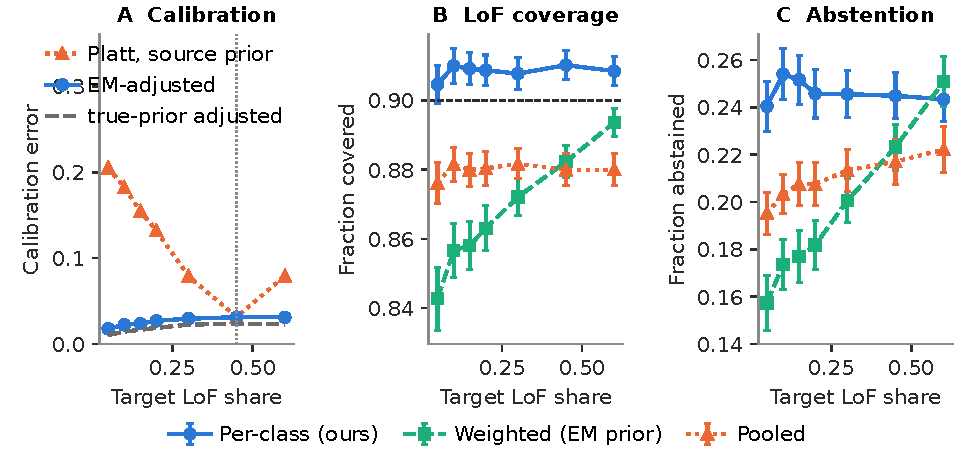
\includegraphics[width=\linewidth]{fig_simulation.pdf}
\caption{Simulation with residue-clustered scores, calibration at LoF share 0.45 and test share on the horizontal axis
(300 replicates; error bars are 95\% intervals of the mean). (A) Expected calibration error of Platt scaling at the
source share, after EM prior adjustment, and after adjustment to the true share. (B) Coverage of LoF variants.
(C) Abstention rate.}\label{fig:sim}
\end{figure}


\paragraph{Why marginal thresholds do not control the minority class.}
A pooled split-conformal threshold $\hat t$ is a quantile of the mixture $\pi_c F_1+(1-\pi_c)F_0$ of the two
class-conditional nonconformity laws, weighted by the calibration share $\pi_c$. Its coverage of class 1 is
$F_1(\hat t)$, which is not controlled; when LoF variants are rare and harder to separate, $F_1(\hat t)<1-\alpha$ while
marginal coverage is still near $1-\alpha$. Reweighting to a known test prior \cite{Podkopaev2021} restores marginal
coverage at that prior but does not control $F_1(\hat t)$ either.


\section{Calibration size, region and gene transfer, and per-gene results}\label{s:practical}
\begin{figure}[ht]
\centering
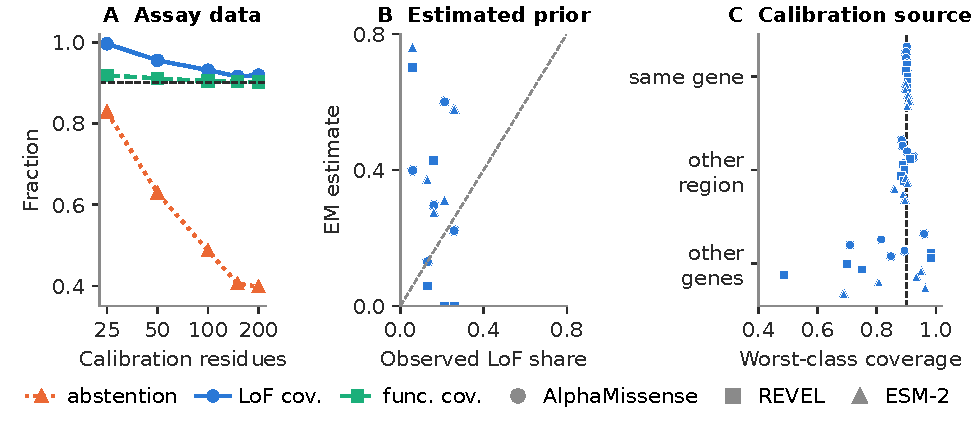
\includegraphics[width=\linewidth]{fig_practical.pdf}
\caption{(A) Coverage and abstention against the number of calibration residues drawn from the gene (mean over genes,
predictors and 50 draws). (B) EM estimate of the LoF share from unlabelled scores against the observed share; the dashed
line is equality. (C) Worst-class coverage when calibrating on random residues of the same gene, on the other three
quarters of the protein, or on the other four genes.}\label{fig:practical}
\end{figure}

 \Cref{tab:app_conformal} gives per gene and predictor the residue-weighted coverage of each
class and the abstention rate of the per-class rule and two baselines; \cref{tab:app_prior} gives the estimated LoF
shares and calibration errors behind \cref{sec:coverage}. When the calibration and test halves of a gene share their LoF
share, label-shift-weighted conformal prediction \cite{Podkopaev2021} with the true share nearly coincides with pooled
conformal; with the EM estimate it inherits the estimation error, which collapsed its LoF coverage in some pairs
(worst-class coverage as low as 0.039 at $\alpha=0.1$).


\begin{table}[ht]
\centering
\caption{Within-gene random split, $\alpha=0.1$, mean of 50 splits. Each cell is residue-weighted LoF coverage /
functional coverage / abstention rate.}\label{tab:app_conformal}
\begin{tabular}{llccc}
\toprule
Predictor & Gene & Per-class (ours) & Pooled conformal & Fixed 0.1/0.9\\
\midrule
AlphaMissense & BRCA1 & 0.916/0.901/0.25 & 0.952/0.889/0.32 & 0.971/0.927/0.44 \\
AlphaMissense & BRCA2 & 0.899/0.903/0.36 & 0.808/0.921/0.17 & 0.890/0.965/0.37 \\
AlphaMissense & BAP1 & 0.909/0.898/0.39 & 0.977/0.880/0.69 & 0.942/0.687/0.26 \\
AlphaMissense & RAD51C & 0.901/0.905/0.17 & 0.824/0.929/0.10 & 0.961/0.973/0.37 \\
AlphaMissense & MSH2 & 0.915/0.901/0.29 & 0.972/0.897/0.70 & 0.956/0.799/0.39 \\
REVEL & BRCA1 & 0.914/0.902/0.34 & 0.962/0.883/0.48 & 0.997/0.999/0.98 \\
REVEL & BRCA2 & 0.912/0.899/0.42 & 0.841/0.911/0.24 & 0.947/0.998/0.68 \\
REVEL & BAP1 & 0.903/0.904/0.42 & 0.545/0.997/0.15 & 0.663/1.000/0.24 \\
REVEL & RAD51C & 0.909/0.904/0.27 & 0.625/0.999/0.20 & 0.680/1.000/0.23 \\
REVEL & MSH2 & 0.911/0.901/0.37 & 0.991/0.896/0.79 & 0.991/0.900/0.80 \\
ESM-2 & BRCA1 & 0.911/0.897/0.37 & 0.912/0.893/0.34 & 0.970/0.975/0.64 \\
ESM-2 & BRCA2 & 0.896/0.903/0.36 & 0.944/0.894/0.51 & 0.964/0.958/0.71 \\
ESM-2 & BAP1 & 0.910/0.905/0.47 & 0.878/0.912/0.36 & 0.903/0.943/0.46 \\
ESM-2 & RAD51C & 0.915/0.908/0.34 & 0.973/0.886/0.50 & 0.987/0.963/0.71 \\
ESM-2 & MSH2 & 0.920/0.902/0.46 & 1.000/0.895/0.80 & 0.993/0.823/0.68 \\
\bottomrule
\end{tabular}
\end{table}

\begin{table}[ht]
\centering
\caption{Prior estimation and calibration on assayed variants outside the ClinVar labelled set. LoF share observed and estimated from
unlabelled scores by expectation--maximization (EM) \cite{Saerens2002} and black-box shift estimation (BBSE) \cite{Lipton2018}; expected calibration error (10 equal-mass
bins) of the ClinVar-Platt posterior, after EM prior adjustment, after adjustment to the true prior, and of Platt
scaling fitted on the other four genes' assay labels. AM: AlphaMissense.}\label{tab:app_prior}
\setlength{\tabcolsep}{4.5pt}
\begin{tabular}{llrrrrrrr}
\toprule
 & & \multicolumn{3}{c}{LoF share} & \multicolumn{4}{c}{Expected calibration error}\\
\cmidrule(lr){3-5}\cmidrule(lr){6-9}
 & & & & & ClinVar & & + true & other\\
Pred. & Gene & obs. & EM & BBSE & Platt & + EM & prior & genes\\
\midrule
AM & BRCA1 & 0.161 & 0.297 & 0.316 & 0.203 & 0.135 & 0.064 & 0.049 \\
AM & BRCA2 & 0.130 & 0.131 & 0.178 & 0.132 & 0.032 & 0.032 & 0.041 \\
AM & BAP1 & 0.213 & 0.601 & 0.588 & 0.341 & 0.388 & 0.255 & 0.119 \\
AM & RAD51C & 0.259 & 0.222 & 0.252 & 0.067 & 0.043 & 0.037 & 0.162 \\
AM & MSH2 & 0.060 & 0.399 & 0.395 & 0.361 & 0.340 & 0.120 & 0.139 \\
REVEL & BRCA1 & 0.161 & 0.429 & 0.336 & 0.285 & 0.268 & 0.058 & 0.140 \\
REVEL & BRCA2 & 0.130 & 0.059 & 0.149 & 0.176 & 0.071 & 0.025 & 0.111 \\
REVEL & BAP1 & 0.213 & 0.000 & 0.000 & 0.092 & 0.213 & 0.149 & 0.138 \\
REVEL & RAD51C & 0.259 & 0.000 & 0.000 & 0.143 & 0.259 & 0.185 & 0.187 \\
REVEL & MSH2 & 0.060 & 0.701 & 0.577 & 0.485 & 0.642 & 0.106 & 0.329 \\
ESM-2 & BRCA1 & 0.161 & 0.276 & 0.304 & 0.212 & 0.114 & 0.050 & 0.044 \\
ESM-2 & BRCA2 & 0.130 & 0.371 & 0.371 & 0.288 & 0.241 & 0.075 & 0.035 \\
ESM-2 & BAP1 & 0.213 & 0.312 & 0.327 & 0.171 & 0.121 & 0.086 & 0.092 \\
ESM-2 & RAD51C & 0.259 & 0.579 & 0.538 & 0.246 & 0.320 & 0.122 & 0.102 \\
ESM-2 & MSH2 & 0.060 & 0.762 & 0.670 & 0.531 & 0.702 & 0.165 & 0.234 \\
\bottomrule
\end{tabular}
\end{table}


\section{Strata, assay-label sensitivity and ClinVar check}\label{s:strata}
For one within-gene split per gene and predictor ($\alpha=0.1$, variant-weighted), coverage of LoF and
functional variants was 0.966 and 0.929 on the third of variants farthest from the assay's class boundary, 0.929 and
0.912 on the middle third, 0.865 and 0.873 on the nearest third, and 0.881 and 0.896 on variants classified VUS in
ClinVar, with abstention rates of 0.334, 0.385, 0.413 and 0.392.


\Cref{tab:app_labels} gives, for each label rule, the number of labelled variants, their LoF share, the coverage and
abstention of the per-class rule, and the oracle check of the certified selection (\cref{sec:transfer}). This analysis
is an independent re-run with its own random splits, so its main-label rows differ from \cref{tab:main} by Monte Carlo
error (for example 0.895 against 0.896 in the lowest pair).

\begin{table}[ht]
\centering
\caption{Sensitivity to the assay-label rule. Each gene is relabelled with the authors' classes or with the control
rule at the stated posterior cut-off; other genes are unchanged. Per-class: lowest mean per-class coverage over the
three predictors (50 random halvings, $\alpha=0.1$); abstention: range over predictors; bounds held: oracle selections
whose certified bound the true likelihood ratio respected (100 draws per predictor); LoF-supp.: share of draws
certifying LoF-supporting calls, range over predictors.}\label{tab:app_labels}
\setlength{\tabcolsep}{4.5pt}
\begin{tabular}{llrrrccc}
\toprule
Gene & Labels & $n$ & LoF & Per-class & Abstention & Bounds held & LoF-supp.\\
\midrule
BRCA2 & controls, 0.80 & 3,971 & 0.136 & 0.894 & 0.49--0.53 & 294/295 & 0.63--0.96 \\
BRCA2 & controls, 0.95 (main) & 3,435 & 0.130 & 0.896 & 0.36--0.42 & 423/423 & 0.90--0.99 \\
BRCA2 & controls, 0.99 & 2,341 & 0.151 & 0.897 & 0.30--0.37 & 591/593 & 0.94--1.00 \\
BAP1 & authors (main) & 4,294 & 0.213 & 0.901 & 0.39--0.47 & 460/460 & 0.90--1.00 \\
BAP1 & controls, 0.95 & 4,221 & 0.100 & 0.899 & 0.13--0.19 & 777/777 & 1.00 \\
RAD51C & authors (main) & 2,225 & 0.259 & 0.895 & 0.18--0.28 & 558/561 & 0.84--0.99 \\
RAD51C & controls, 0.95 & 832 & 0.538 & 0.902 & 0.07--0.19 & 868/868 & 0.98--1.00 \\
\bottomrule
\end{tabular}
\end{table}


\Cref{tab:app_clinvar} gives the exploratory check of the calls against ClinVar labels (\cref{sec:evidence}),
per gene and pooled. Only BRCA1, BRCA2 and MSH2 have enough labelled residues for informative bounds; across them the
LoF-call lower bounds differ by gene, so the pooled values should not be read as a common likelihood ratio. Some ClinVar
classifications already use these assays or predictors as evidence, so this check is not independent clinical
validation.

\begin{table}[ht]
\centering
\caption{Calls judged against ClinVar labels (exploratory). Thresholds ($\alpha=0.1$) are set on each gene's assay
labels; one ClinVar variant with $\ge$2 stars is kept per residue. $n$: kept P/LP and B/LB variants; calls: LoF (or
functional) calls among P/LP / among B/LB variants; $L^+$, $U^-$: likelihood-ratio bounds from one-sided
Clopper--Pearson endpoints at level 0.025 each (simultaneous level 0.95 per ratio). Pooled rows sum the kept counts over
genes, each gene with its own thresholds. BAP1 and RAD51C have too few labelled residues to be informative.}
\label{tab:app_clinvar}
\setlength{\tabcolsep}{4.5pt}
\begin{tabular}{llrrcrcr}
\toprule
Pred. & Gene & $n$ P/LP & $n$ B/LB & LoF calls & $L^+$ & func.\ calls & $U^-$\\
\midrule
AM & BRCA1 & 75 & 170 & 56/1 & 19.6 & 8/153 & 0.24 \\
AM & BRCA2 & 60 & 210 & 49/8 & 9.44 & 6/164 & 0.29 \\
AM & BAP1 & 6 & 8 & 5/0 & 0.97 & 1/8 & 1.02 \\
AM & RAD51C & 8 & 3 & 5/1 & 0.27 & 2/2 & 6.90 \\
AM & MSH2 & 72 & 55 & 50/6 & 2.58 & 9/46 & 0.31 \\
AM & pooled & 221 & 446 & 165/16 & 11.9 & 26/373 & 0.21 \\
REVEL & BRCA1 & 75 & 170 & 48/10 & 4.94 & 8/134 & 0.28 \\
REVEL & BRCA2 & 60 & 210 & 44/9 & 7.56 & 11/182 & 0.37 \\
REVEL & BAP1 & 6 & 8 & 4/0 & 0.60 & 2/8 & 1.23 \\
REVEL & RAD51C & 8 & 3 & 6/0 & 0.49 & 2/3 & 2.23 \\
REVEL & MSH2 & 72 & 55 & 43/3 & 3.14 & 5/38 & 0.28 \\
REVEL & pooled & 221 & 446 & 145/22 & 7.99 & 28/365 & 0.23 \\
ESM-2 & BRCA1 & 75 & 170 & 47/1 & 15.7 & 10/159 & 0.26 \\
ESM-2 & BRCA2 & 60 & 210 & 33/4 & 8.66 & 9/184 & 0.32 \\
ESM-2 & BAP1 & 6 & 8 & 5/0 & 0.97 & 1/5 & 2.62 \\
ESM-2 & RAD51C & 8 & 3 & 5/0 & 0.35 & 1/1 & 62.7 \\
ESM-2 & MSH2 & 72 & 55 & 44/3 & 3.23 & 3/33 & 0.25 \\
ESM-2 & pooled & 221 & 446 & 134/8 & 15.4 & 24/382 & 0.19 \\
\bottomrule
\end{tabular}
\end{table}


\section{Implementation}\label{s:impl}
Inputs: ClinVar \nolinkurl{variant_summary.txt.gz} of 26 October 2026 (SHA-256 in \nolinkurl{data/MANIFEST.txt});
MaveDB score sets \nolinkurl{urn:mavedb:00000097-0-2} (BRCA1), \nolinkurl{00001279-a-1} (BRCA2), \nolinkurl{00000662-0-1}
(BAP1), \nolinkurl{00000673-0-1} (RAD51C) and \nolinkurl{00000050-a-1} (MSH2, positive scores = loss of function); Ensembl VEP
REST on GRCh38 (release 116) with the AlphaMissense and REVEL annotations; ESM-2 \nolinkurl{esm2_t33_650M_UR50D}.
Distance from the class boundary is the absolute difference between a variant's assay score
and the midpoint of the two class medians in its gene, divided by the distance between the medians. Expected calibration
error uses ten equal-mass bins. AUROC intervals are percentiles of 1,000 bootstrap resamples of residues. The region split
divides each gene's assayed residues into four contiguous blocks with equal numbers of distinct positions. ClinVar records
whose aggregate germline classification is empty (somatic-only submissions) are treated as unclassified. All random
draws use NumPy generators with fixed seeds (2027 plus a fixed offset per experiment). The experiments run on a laptop CPU with Python 3.13, NumPy 2.5,
SciPy 1.18, scikit-learn 1.9 and pandas 3.1; ESM-2 scoring used fair-esm 2.0 and PyTorch 2.14 on an Apple-silicon GPU.
Exact versions and data checksums are in the repository. The Platt map is checked to be increasing (positive
slope) every time it is fitted, and every fit in the experiments passed. Certified bounds use the conventions of
Section 3: $U^-=\infty$ when $\ell_{\mathrm{TN}}=0$, an empirical ratio $x/0$ is $\infty$ for $x>0$, and $0/0$ is
undefined (never a claim); boundary cases are covered by unit tests (\texttt{make test}). The VUS-shift LoF shares
are residue-weighted for both the calibration sample (one variant per residue) and the VUS (each residue weighted
equally, then its variants).
